\documentclass{article}
\usepackage{graphicx}

\begin{document}

\title{Monte Carlo, Exercise Session 3}
\author{Alexey Sofiev, 013573003}

\maketitle

%\begin{abstract}
%The abstract text goes here.
%\end{abstract}

\section{Exercise 1}
Code: Ex1.cpp. Answer: Figure \ref{fig:ex1_answer}.

\begin{figure}[!hbt]
    \centering
    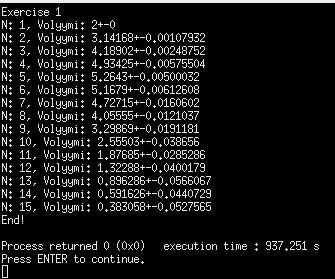
\includegraphics[width=4.3in]{ex1_answer}
    \caption{Ex1 answer.}
    \label{fig:ex1_answer}
\end{figure}

	Result makes sense, since the correct answers are 2, $\pi$, 4*$\pi$/3 ...


\section{Exercise 2}
Answer presented in Figure \ref{fig:ex2_answer}.
\begin{figure}[!hbt]
	\centering
	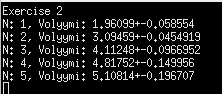
\includegraphics[width=4.3in]{ex2_answer}
	\caption{Ex2 answer.}
	\label{fig:ex2_answer}
\end{figure}

Result in Exercise 1 and Exercise 2 are pretty similar. However the sampling method requires significantly more time, so had to increase binning, which increased the uncertainty.


\section{Conclusion}
Write your conclusion here.

\end{document}